%%
%% copyright quintard julien
%% 
%% kaneton
%% 
%% k4-subject.tex
%% 
%% path          /root/data/research/projects/svn/kaneton/projects/k4
%% 
%% made by mycure
%%         quintard julien   [quinta_j@epita.fr]
%% 
%% started on    Sat Feb 26 15:06:05 2005   mycure
%% last update   Fri Mar 18 12:57:18 2005   mycure
%%

\documentclass[10pt,a4wide]{article}
\usepackage[english]{babel}
\usepackage{a4wide}
\usepackage{graphicx}
\usepackage{graphics}
\usepackage{fancyheadings}
\pagestyle{fancy}

\bibliographystyle{plain}

\lhead{\scriptsize{kaneton project}}
\rhead{k4 subject}
\rfoot{\scriptsize{EPITA System Lab}}

\title{kaneton4}

\author{Julien Quintard - \small{quinta\_j@epita.fr} \\
        Jean-Pascal Billaud - \small{billau\_j@epita.fr} \\ \\
	\small{last updated by} \\
	Julien Quintard - \small{quinta\_j@epita.fr}}

\date{\today}

\begin{document}
\maketitle

\section{Informations}

\begin{tabular}{p{7cm}l}

Date de rendu: & Lundi XXX Mars 2005 \`a 23h42 \\
Dur\'ee du projet: & XXX semaines \\
Nom du fichier de rendu: & k4.tar.gz \\
Responsable du projet: & Julien Quintard - \small{quinta\_j@epita.fr} \\
                       & Jean-Pascal Billaud - \small{billau\_j@epita.fr} \\
Newsgroups d\'edi\'es: & epita.kaneton, epita.adm.sr \\
Langages: & asm, C \\
Architectures: & Intel 32-bit \\
Nombre de personnes par groupes: & 3 \`a 5

\end{tabular}

\section{Introduction}

\paragraph{}

La gestion de la m\'emoire \'etant disponible, votre kernel est capable
d'allouer de la m\'emoire, que celle-ci soit physique ou bien virtuelle
et si besoin est de la mapp\'ee.

\paragraph{}

Votre kernel dispose de presque toutes les fonctionnalit\'es mises \`a part
une gestion des t\^aches et une gestion des communications inter-processus.

\paragraph{}

Le but de ce projet est donc de fournir une interface pour la gestion
des processus, des threads mais \'egalement le n\'ec\'essaire pour pouvoir
ordonnancer les fils d'ex\'ecution.

\section{Travail Demand\'e}

\paragraph{}

XXX

\section{Nomenclature}

\paragraph{}

Avant toute chose il est important de bien d\'efinir les diff\'erents
termes que nous utiliserons dans ce document. Pour \^etre plus pr\'ecis
nous allons expliciter les termes utilis\'es pour d\'efinir les
diff\'erents types de t\^aches:

\paragraph{}

\subsection{Module}

\paragraph{}

Un \textbf{module} est une entit\'e particuli\`ere car celle-ci est passive.
En effet un module en soit ne vit pas, ne s'ex\'ecute pas. Un module
est un ex\'ecutable stock\'e en m\'emoire principale plus ou moins longuement
dans le temps. Par exemple les ex\'ecutables des services ou drivers, bref
des t\^aches fondamentales, seront sauvegarder constamment en m\'emoire
principale afin que celles-ci puissent \^etre lanc\'ees ou relanc\'ees
tr\`es rapidement et sans aide quelconque.

\subsection{User}

\paragraph{}

Une t\^ache de type \textbf{user} est consid\'er\'e comme l'entit\'e ayant
les droits les plus faible au niveau syst\`eme. D'un point de vue concret
c'est tout ce que nous nommont ``userland'': les programmes utilisateurs.

\subsection{Service}

\paragraph{}

Un \textbf{service} est une t\^ache qui comme son nom l'indique fournit
un service. En d'autres termes, ce type de t\^ache est appell\'e par
les taches du m\^eme niveau ou inf\'erieur pour effectuer une op\'eration
sp\'ecifique nomm\'ee \textbf{service}.

\subsection{Driver}

\paragraph{}

Un \textbf{driver} est un service particulier dans le sens ou celui-ci
interagit avec le mat\'eriel. Cela ne signifie pas qu'il a des droits
accrus. En effet g\'en\'eralement, le kernel, les drivers et les services
auront concr\`etement les m\^eme droits syst\`emes.

\subsection{Kernel}

\paragraph{}

Pour finir, le \textbf{kernel} est une sorte de super-driver car celui-ci
fournit un service en ayant acc\`es \`a tous les p\'eriph\'eriques mais
\'egalement \`a toutes les structures internes.

\section{Priorit\'e}

\paragraph{}

Les t\^ache peuvent \^etre diff\'erenci\'ees par leurs comportements. Pour
cette raison chaque classe se voit associer un comportement \textbf{t\_behav}.
Ce comportement identifie un interval de priorit\'e pour la t\`ache, celle-ci
pouvant \'evoluer librement dans cet interval.

\paragraph{}

Comme nous venons de le dire la t\^ache peut donc retoucher sa priorit\'e.
Pour r\'esumer une t\^ache est toujours associ\'ee \`a: un comportement
\textbf{t\_behav} identifiant le degr\'e de priorit\'e d\'esir\'e et
une priorit\'e courante \textbf{t\_prior} celle-ci \'etant constamment
situ\'ee dans l'interval associ\'e au comportement.

\paragraph{}

Voici les diff\'erents comportements qu'une t\^ache peut prendre:

\begin{center}

\begin{tabular}{|p{4cm}|p{4cm}|p{4cm}|}

\hline

\textbf{behaviour}	& \textbf{interval}	& \textbf{default priority} \\

\hline

KERNEL			& 100 - 120		& 110 \\

\hline

REALTIME		& 80 - 100		& 90 \\

\hline

INTERACTIVE		& 60 - 80		& 70 \\

\hline

TIMESHARING		& 30 - 60		& 45 \\

\hline

BACKGROUND		& 10 - 30		& 20 \\

\hline

\end{tabular}

\end{center}

Le type \textbf{behav} ne d\'efinit que la priorit\'e de la t\^ache vis-\`a-vis
de l'ordonnanceur mais bien l'interval dans lequel la t\^ache va pouvoir
\'evoluer.

\paragraph{}

L'ordonnanceur pour pouvoir correctement d\'ecider du temps a attribuer \`a
chaque t\^ache suivant sa priorit\'e doit garder un certain nombre de
valeurs constamment \`a jour notamment: le nombre de t\^aches actuellement
sur le syst\`eme et le quantum de temps \`a attribuer \`a une t\^ache.

\paragraph{}

Avec ces deux param\`etre l'ordonnanceur sera capable de calculer le temps
processeur \`a attribuer \`a chaque t\^ache en fonction de sa priorit\'e.

\section{Classe}

\paragraph{}

En plus d'avoir un comportement et une priorit\'e courante, chaque
t\^ache se voit attribuer une \textbf{classe} lors de sa cr\'eation.

\paragraph{}

Cette \textbf{classe} d\'efinit les droits g\'en\'eraux de la t\^ache
vis-\`a-vis du syst\`eme.

\paragraph{}

Les diff\'erentes classes de t\^aches sont les suivantes: CLASS\_KERNEL,
CLASS\_DRIVER, CLASS\_SERVICE, CLASS\_USER.

\paragraph{}

Le fait d'appartenir \`a telle ou telle classe ne signifie rien mis \`a
part que dans certaines classes vous pouvez effectuer certaines op\'erations
privil\'egi\'ees.

\paragraph{}

De plus, ces classes permettent de classifier les t\^aches, ceci \'etant
obligatoire pour pouvoir \'etablir un syst\`eme hi\'erarchis\'e.

\subsection{Visualisation}

\paragraph{}

Voici une visualisation des couches de classes de t\^aches.

\paragraph{}

\begin{figure}[h]
\centerline{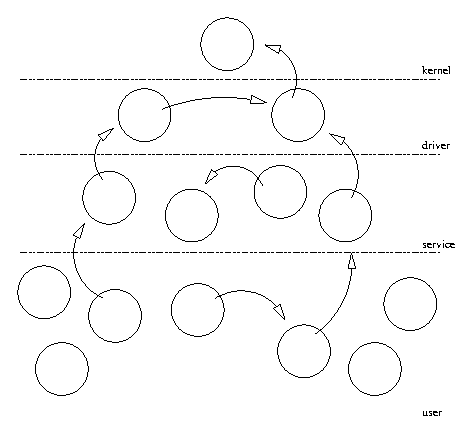
\includegraphics{figures/classes.eps}}
\end{figure}

\paragraph{}

\`A noter que les appels entre les couches sont normalis\'es pour coller
au syst\`eme hi\'erarchique. Les t\^aches peuvent appeller une t\^ache
disposant de privil\`eges sup\'erieur ou \'egaux aux siens.

\paragraph{}

Ce syst\`eme hi\'erarchique doit absolument \^etre suivi concernant la
demande de service. Par exemple un processus peut demander \`a un service
ou au kernel de faire quelque chose pour lui. En revanche il n'arrivera jamais
que le kernel demande \`a un driver de faire quelque chose pour lui.

\section{Interfaces}

\paragraph{}

Voici les interfaces \`a suivre pour ce projet.

\subsection{Ordonnanceur}

\paragraph{}

L'interface de l'ordonnanceur est simple mais permet n\'eanmoins la gestion
de priorit\'es sur les tasks comme sur les threads.

\paragraph{}

\`A noter que le gestionnaire de t\^aches, le gestionnaire de threads et
l'ordonnanceur \'evoluent ensemble et modifient tous la structure principale
de l'ordonnanceur pour maintenant l'ordonnancement \`a jour en ce qui
concerne les priorit\'es par exemple.

\paragraph{}

\hspace{1.5cm}int \textbf{sched\_init}(t\_quantum \textbf{quantum});

\paragraph{}

Cette fonction initialise l'ordonnanceur en lui sp\'ecifiant le quantum
de temps par d\'efaut allou\'e \`a chaque processus.

\paragraph{}

Pour b\'en\'eficier d'avantage de temps d'ex\'ecution les processus
peuvent faire \'evoluer leurs priorit\'es.

\paragraph{}

\hspace{1.5cm}int \textbf{sched\_quantum}(t\_quantum \textbf{quantum});

\paragraph{}

Cette fonction permet de red\'efinir le quantum de temps allou\'e
aux processus.

\paragraph{}

Pour ceux ayant fait un fichier de configuration, il serait int\'eressant
de sp\'ecifier dans ce fichier de configuration le quantum par d\'efaut.

\paragraph{}

\hspace{1.5cm}int \textbf{sched\_yield}(void);

\paragraph{}

Cette fonction permet \`a la t\^ache l'utilisant de redonner la main
\textbf{volontairement} \`a l'ordonnanceur. Cela n'arrive \'evidemment
que lorsque la t\^ache se retrouve bloqu\'ee et que celle-ci pr\'ef\`ere
se d\'egager de son temps processeur car inutilis\'e.

\paragraph{}

\hspace{1.5cm}int \textbf{sched\_next}(t\_thrid* \textbf{thrid});

\paragraph{}

Cette fonction se contente de retourner dans la variable \textbf{thrid}
l'identifiant du prochain thread \`a ex\'ecuter.

\paragraph{}

\hspace{1.5cm}int \textbf{sched\_switch}(t\_thrid \textbf{thrid});

\paragraph{}

Cette fonction \'effectue la changement de contexte et charge donc le contexte
du thread \textbf{thrid} afin de l'ex\'ecuter.

\paragraph{}

Pensez \`a suivre les indications expliqu\'ees en cours pour pouvoir
ex\'ecuter un changement de contexte sans probl\`emes tout en restant
portable.

\paragraph{}

\hspace{1.5cm}int \textbf{sched\_tskid}(t\_tskid* \textbf{tskid});

\paragraph{}

Cette fonction remplie l'argument \textbf{tskid} avec l'identifiant de
la t\^ache en cours d'ex\'ecution.

\paragraph{}

\hspace{1.5cm}int \textbf{sched\_thrid}(t\_thrid* \textbf{thrid});

\paragraph{}

Cette fonction remplie l'argument \textbf{thrid} avec l'identifiant du
thread en cours d'ex\'ecution.

\paragraph{}

\hspace{1.5cm}int \textbf{sched\_clean}(void);

\paragraph{}

Cette fonction r\'einitialise l'ordonnanceur.

\subsection{Espace d'adressage}

\paragraph{}

L'interface d'espaces d'adressage doit \^etre modif\'ee pour pouvoir
s'int\'egrer avec les nouveaux composants.

\paragraph{}

Dans un premier temps, un champ doit \^etre ajout\'e \`a la structure
\textbf{t\_as}. La structure \textbf{t\_as} devrait d\'esormais ressembler \`a
cela:

\begin{verbatim}
typedef struct          s_as
{
  t_asid                asid;
  t_tskid               tskid;

  [pas_data_structure]  pas;
  [vas_data_structure]  vas;
}                       t_as;
\end{verbatim}

\paragraph{}

En effet ce champ va nous permettre de savoir si l'espace d'adressage
est bien li\'e \`a un processus ou si au contraire il est encore
isol\'e.

\paragraph{}

Ensuite il va vous falloir ajouter deux fonctionnalit\'es \`a votre
interface de gestion d'espaces d'adressage.

\paragraph{}

\hspace{1.5cm}int \textbf{as\_attach}(t\_tskid \textbf{tskid},
                                      t\_asid \textbf{asid});

\paragraph{}

Cette fonction attache un espace d'adressage \`a une t\^ache.

\paragraph{}

\hspace{1.5cm}int \textbf{as\_detach}(t\_tskid \textbf{tskid},
                                      t\_asid* \textbf{asid});

\paragraph{}

Cette fonction d\'etache un espace d'adressage d'une t\^ache, la variable
\textbf{asid} recevant l'asid de l'espace d'adressage d\'etach\'e.

\subsection{Cpu}

\paragraph{}

Le gestionnaire de processeurs ne sera pas \'etudi\'e en d\'etail. N\'eanmoins
il sera int\'eressant de cr\'eer une \'ebauche d'interface pour plus tard.
De plus certains bonus viendront se greffer dans ce gestionnaire.

\paragraph{}

\hspace{1.5cm}int \textbf{cpu\_init}(void);

\paragraph{}

Cette fonction initialise le gestionnaire de processeurs.

\paragraph{}

\hspace{1.5cm}int \textbf{cpu\_clean}(void);

\paragraph{}

Cette fonction r\'einitialise le gestionnaire de processeurs.

\subsection{Task}

\paragraph{}

Vous devez fournir une interface compl\`ete pour la gestion des t\^aches.
\textbf{kaneton} ne dispose pas de \textbf{processus} au sens UNIX, n\'eanmoins
nous utiliserons parfois ce terme pour d\'esigner une t\^ache.

\paragraph{}

Une t\^ache est une entit\'e compos\'ee de fils d'ex\'ecutions et de
m\'emoire.

\paragraph{}

Le processus de cr\'eation de task se d\'ecoupe en trois phases:

\begin{enumerate}

\item r\'eservation d'une structure \textbf{t\_task}

\item attachement d'un espace d'adressage \`a la t\^ache

\item attachement d'un thread \`a la t\^ache.

\end{enumerate}

La derni\`ere \'etape peut \^etre r\'ep\'et\'ee autant de fois que voulue.

\paragraph{}

La particularit\'e d'un tel syst\`eme est son extr\^eme modularit\'e. Avec
celui-ci il est possible de cr\'eer tous les espaces d'adressages puis
de les attacher \`a la toute fin.

\paragraph{}

De plus il est possible de d\'etacher un espace d'adressage ou m\^eme
des threads pour les r\'e-attacher \`a d'autres t\^aches, tout cela
facilitant \'enorm\'ement le recyclage de structures internes aux
kernel: \textbf{t\_as}, \textbf{t\_thread}, \textbf{t\_task} etc..

\paragraph{}

Voyons d\'esormais l'interface du gestionnaire de t\^aches.

\paragraph{}

\hspace{1.5cm}int \textbf{task\_init}(void);

\paragraph{}

Cette fonction initialise le gestionnaire de t\^aches.

\paragraph{}

\hspace{1.5cm}int \textbf{task\_rsv}(t\_class \textbf{class},
                                     t\_behav \textbf{behav},
                                     t\_prior \textbf{prior},
                                     t\_tskid* \textbf{tskid});

\paragraph{}

Cette fonction r\'eserve  et initialise une t\^ache. L'argument
\textbf{tskid} se voit attribu\'e l'identifiant de la t\^ache cr\'e\'ee.

\paragraph{}

L'argument \textbf{class} repr\'esente la classe de la t\^ache:
CLASS\_KERNEL, CLASS\_DRIVER, CLASS\_SERVICE et CLASS\_USER.

\paragraph{}

L'argument \textbf{behav} repr\'esente le comportement, que nous avons
d\'ej\`a vu au d\'ebut de ce document: BEHAV\_KERNEL, BEHAV\_REALTIME,
BEHAV\_INTERACTIVE, BEHAV\_TIMESHARING et BEHAV\_BACKGROUND.

\paragraph{}

L'argument \textbf{prior} repr\'esente la priorit\'e de la t\^ache:
PRIOR\_KERNEL, PRIOR\_REALTIME, PRIOR\_INTERACTIVE, PRIOR\_TIMESHARING,
PRIOR\_BACKGROUND repr\'esentent les priorit\'es par d\'efaut des
comportement portant le m\^eme nom.

\paragraph{}

\hspace{1.5cm}int \textbf{task\_clone}(t\_tskid \textbf{old},
                                       t\_tskid \textbf{new});

\paragraph{}

Cette fonction se charge de dupliquer une t\^ache. Attention il faut dupliquer
chaque \'el\'ement de cette structure comme par exemple, l'espace d'adressage,
les threads mais \'eglament tous les \'el\'ements qui seront ajout\'es plus
tard comme par exemple les identifiants de fichiers ouverts en appellant
certainement une routine du type: \textbf{vfs\_clone}().

\paragraph{}

\hspace{1.5cm}int \textbf{task\_getprior}(t\_tskid \textbf{tskid},
                                          t\_prior* \textbf{prior});

\paragraph{}

Cette fonction retourne dans \textbf{prior} la priorit\'e courante
de la t\^ache. Cette fonction est utile pour ensuite recalculer une
nouvelle priorit\'e pour finir par la mettre \`a jour.

\paragraph{}

\hspace{1.5cm}int \textbf{task\_setprior}(t\_tskid \textbf{tskid},
                                          t\_prior \textbf{prior});

\paragraph{}

Cette fonction met \`a jour la priorit\'e de la t\^ache.

\paragraph{}

\hspace{1.5cm}int \textbf{task\_wait}(t\_tskid \textbf{tskid},
                                      t\_wait* \textbf{wait});

\paragraph{}

Cette fonction est relativement identique \`a la fonction \textbf{wait}()
d'UNIX.

\paragraph{}

Son r\^ole est de bloquer la t\^ache appellante jusqu\`a ce que la
t\^ache \textbf{tskid} meurt; l'argument \textbf{wait} contenant des
informations sur la t\^ache venant de terminer: qui, comment, pourquoi etc..

\paragraph{}

\`A noter que l'argument \textbf{wait} peut \^etre sp\'ecifi\'e \`a NULL
si jamais la t\^ache qui effectue le \textbf{task\_wait}() ne d\'esire
pas obtenir d'informations sur la t\^ache d\'ec\'ed\'ee.

\paragraph{}

Attention, vous devez suivre le m\^eme protocole qu'UNIX. Si un
\textbf{task\_wait}() est effectu\'e sur une t\^ache d\'ej\`a morte -
\'etat zombie - la fonction retourne directement. Pensez bien qu'apr\`es
la mort d'une t\^ache, celle-ci passe en \'etat zombie et que cet \'etat
dure jusqu'\`a ce qu'une t\^ache effectue un \textbf{task\_wait}(). Une fois
le \textbf{task\_wait}() effectu\'e la t\^ache morte est recycl\'ee
et ses ressources lib\'er\'ees.

\paragraph{}

L'argument \textbf{tskid} peut prendre deux valeurs significatives:

\begin{itemize}

\item Une \textbf{valeur sup\'erieure \`a z\'ero} qui correspond au taskid de
      la t\^ache \`a observer.

\item \textbf{Z\'ero} qui correspond \`a ``n'importe quel fils''. Bien entendu
      dans ce cas pr\'ecis il sera int\'eressant d'explorer la variable
      \textbf{t\_wait} pour conna\^itre l'identit\'e de la t\^ache venant
      de mourir.

\end{itemize}

\paragraph{}

Pour plus d'informations \`a propos du type \textbf{t\_wait} et des
informations qu'il contient, r\'ef\'erez vous \`a la section Types.

\paragraph{}

\hspace{1.5cm}int \textbf{task\_rel}(t\_tskid \textbf{tskid});

\paragraph{}

Cette fonction lib\`ere la structure task. Attention, la fonction
devra se charger de lib\'erer l'espace d'adressage et les threads
si ceux-ci sont encore attach\'es \`a la t\^ache lors de sa lib\'eration.

\paragraph{}

\hspace{1.5cm}int \textbf{task\_ptskid}(t\_tskid \textbf{tskid},
                                        t\_tskid* \textbf{ptskid});

\paragraph{}

Cette fonction remplie l'argument \textbf{ptskid} avec l'identifiant de
la t\^ache parente de la t\^ache \textbf{tskid}.

\paragraph{}

\hspace{1.5cm}int \textbf{task\_asid}(t\_tskid \textbf{tskid},
                                      t\_asid* \textbf{asid});

\paragraph{}

Cette fonction remplie l'argument \textbf{asid} avec l'identifiant de
l'espace d'adressage de la t\^ache \textbf{tskid}.

\paragraph{}

\hspace{1.5cm}int \textbf{task\_run}(t\_tskid \textbf{tskid});

\paragraph{}

Cette fonction active la t\^ache \textbf{taskid} comme \'etant ex\'ecutable.

\paragraph{}

\hspace{1.5cm}int \textbf{task\_stop}(t\_tskid \textbf{tskid});

\paragraph{}

Cette fonction arr\^ete la t\^ache \textbf{tskid}.

\paragraph{}

Bien entendu ces deux derni\`eres fonctions n\'ecessitent soit
d'\^etre le kernel, soit d'\^etre la t\^ache en question ou bien d'en
\^etre le parent sans quoi une erreur sera retourn\'ee.

\paragraph{}

De plus une fonction ne pourra devenir ex\'ecutable si jamais aucun
thread ou aucun espace d'adressage n'est attach\'e \`a celle-ci.

\paragraph{}

\hspace{1.5cm}int \textbf{task\_clean}(void);

\paragraph{}

Cette fonction r\'einitialise le gestionnaire de t\^aches.

\subsection{Thread}

\paragraph{}

Voyons d\'esormais l'interface du gestionnaire de threads.

\paragraph{}

\hspace{1.5cm}int \textbf{thread\_stop}(t\_tskid \textbf{tskid});

XXX

\section{Types}

XXX

\subsection{Bonus}

\paragraph{}

Voici les bonus pour ce projet

\subsubsection{Cpu detection}

\paragraph{}

Comme le titre l'indique, le but de ce bonus est de d\'etecter et r\'ecup\'erer
toutes les informations relatives au processeur: mod\`ele, puissance etc..

\paragraph{}

Lors de l'appel \`a l'initialisation du CPU, dans la fonction
\textbf{cpu\_init}(), il vous sera demander d'afficher les informations
recolt\'ees.

XXX

\begin{verbatim}

----- types

t_task
{
  tskid tskid
  asid asid;

  tskid parent;

  t_class class; /* classe de la tache: KERNEL, DRIVER, SERVICE, USER */
  t_prior prior; /* priorite courante cf: plus haut */
  t_cpu cpu;

  t_status schedstatus; /* SCHED_STATUS_: SLEEP, RUN, STOP, ZOMBIE */
  t_status tskstatus; /* RUN, WAITING, IO etc... */
  t_status waitstatus; /* rempli quand la tache meurt */

  thrid current; /* thread en cours d execution */

  uint32 nthreads;
  thrid threads; /* liste de threads */
}

queues:
  run
  zombies
  sleep
  stop

t_thread
{

}

t_tskid
t_thrid
t_quantum
t_class
t_status (wait)
t_prior
t_cpu CPU_ANY, CPU_0 (bsp bootstrap processor) CPU_1 ...
t_waitstatus 16-bit
t_wait
{
  t_tskid tskid; /* la tache qui vient de mourir */
  t_waitstatus status; /* etat de la tache morte */
}

status: [6-bit reserved][2-bit status][8-bit exit/terminate-code]

WAIT_STATUS_MASK	0x0300
WAIT_VALUE_MASK		0x00ff

WAIT_TSKID(wait)
  wait.tskid
	returns the child id which causes the task to unblock

WAIT_STATUS(wait)
  wait.status & WAIT_STATUS_MASK
	returns the child status: exited or forced to terminate

WAIT_VALUE(status)
  wait.status & WAIT_VALUE_CODE
	returns the status returned when exited or the code describing
	the error which occured and forced the child to terminate

#define WAIT_EXITED		0x0 << 8
#define WAIT_TERMINATED		0x1 << 8

----- sched

(*) le kernel doit garder en memoire:
	. a) le nombre de processes en cours
	. b) la somme des priorites des processes
	. c) le quantum actuel

	-> quantum total = a * c
	-> quantum du process = priority * quantum total / b

(*) le process doit garder en memoire:
	. d) le nombre de threads
	. e) la somme des priorites des threads

	-> quantum du thread = priority * quantum du process / e

(*) si le quantum d'un process descend en dessous du seuil de la classe
    inferieure c'est que ca commence a devenir tendu et la par exemple
    on pourrait envisager sur un systeme distribue a migrer des processus
    et a lancer les nouveaux processus sur une autre machine.

name lprior hprior default

KERNEL 100 - 120 default=110
REALTIME 80 - 100 default=90
INTERACTIVE 60 - 80 default=70
TIMESHARING 30 - 60 default=45
BACKGROUND 10 - 30 default=20

WARNING: division d'entiers donc avec 0 ca peut foutre la merde

5 tasks avec une somme de priorites de 276 avec 20ms par defaut par processus
soit 20*5=100ms pour tout le monde:
	1) B 15
	2) R 100
	3) T 33
	4) T 58
	5) I 70

IL FAUT DONC TJS GARDER LA SOMME DES PRIORITES DES PROCESSUS

1) 15*100/276	=	5.4		/* a calculer en ticks apres */
2) 100*100/276	=	36.2
3) 33*100/276	=	11.9
4) 58*100/276	=	21.0
5) 70*100/276	=	25.3

			99.8

sched_init(quantum); /* pas besoin de mettre de classe par defaut, le classe
			par defaut c'est TIMESHARING avec la priorite par
			defaut de cette classe. ensuite ben il suffit
			d'utiliser le fichier de conf et hop on peut les
			redefinir */

sched_next(cpu, *thrid);
		/* cpu: CPU_3, CPU_4 ... example: CPU_3 default: CPU_ANY
		    if nothing found */

sched_prior(tskid, prior); /* class check and then update priority */

sched_yield(void); /* redonne la main au scheduler volontairement */

sched_quantum(quantum); /* modifie le quantum de temps */

/* XXX modifier la frequence */

sched_clear();

----- cpu

cpu_init(); /* detection du cpu etc... BONUS */

cpu_add(cpu, thrid); /* CPU_0, CPU_1 ... limite a 32 CPUs si cpu 32-bit */
			   /* par defaut CPU_ANY est mis */
cpu_rem(cpu, thrid);

cpu_clean();

----- task

Le but de toutes les fonctions est de rendre le code extremement simple
comme le demontre task_create() et l'emulation de fork(); d'ailleurs
ces fonctions pourrraient faire office de tests.

task_init();

task_rsv(t_class class, t_prior prior, t_tskid* tskid);

class: CLASS_KERNEL, CLASS_DRIVER, CLASS_SERVICE, CLASS_USER

          default              low               high

prior: PRIOR_KERNEL => LPRIOR_KERNEL, HPRIOR_KERNEL
       PRIOR_REALTIME => LPRIOR_REALTIME, HPRIOR_REALTIME
       PRIOR_INTERACTIVE => LPRIOR_INTERACTIVE, HPRIOR_INTERACTIVE
       PRIOR_TIMESHARING => LPRIOR_TIMESHARING, HPRIOR_TIMESHARING
       PRIOR_BACKGROUND => LPRIOR_BACKGROUND, HPRIOR_BACKGROUND

#define PRIOR_LOW(_prior_) \
  L##_prior_

#define PRIOR_HIGH(_prior_) \
  H##_prior_

mettre des valeurs fixes pour que les programmes puissent changer leurs
priorites. ces valeurs ne doivent pas etre modifiees par le fichier de conf.
juste le quantum dans le fichier de conf.

par defaut, lors de la creation d'une task elle est marque comme STOPPED

task_prior(tskid, *prior); /* get current priority, useful with PRIOR_DEFAULT*/

task_rel(t_tskid tskid);

task_load(t_tskid tskid, t_thrid thrid, t_modid modid);
	-> mod_get
	-> init thrid

task_unload(t_tskid tskid);

pour pouvoir faire l'unload correctement il faut garder

XXX
task_create(t_modid modid, t_class class, t_tskid *tskid)
{
  t_tskid tskid;
  t_asid  asid;
  t_thrid thrid;
  t_vaddr entry;

  task_rsv(class, PRIOR_TIMESHARING, &tskid);

  as_rsv(&asid);
  as_attach(tskid, asid);

  thread_rsv(&thrid);
  thread_attach(tskid, asid);

  thread_stack(thrid, THREAD_STACKSZ); /* 1 page de stack ??? comment ??? */

  mod_entry(modid, &entry);
  thread_pc(thrid, entry);

  /*
   * if we wanted another thread
   */
  /*
   {
     t_thrid another;

     thread_rsv(&another);
     thread_attach(tskid, another);

     thread_stack(thrid, 9); /* fonction extremement recursive donc 9 pages */

     my_function_which_find_a_special_entry_parsing_elf_header(modid, &entry);

     thread_pc(thrid, entry);
   }
  */

  task_run(tskid);
}
XXX
fork()
{
  t_tskid task;
  t_cpu cpu;

  t_tskid tskid;
  t_thrid thrid;
  t_asid  asid;

  cpu_current(&cpu);
  sched_current(cpu, &task);

  task_asid(current, &asid); /* get as id */
  task_thrid(current, &thrid); /* get current thread id */

  task_rsv(CLASS_KERNEL, PRIOR_KERNEL, &tskid);

  as_clone(asid, &asid);
  as_attach(tskid, asid);

  thread_clone(thrid, &thrid); /* on decide de ne cloner qu'un thread,
				  celui qui appelle fork: le courant */
  thread_attach(tskid, thrid);

  task_run(tskid);
}
XXX

task_wait(tskid, t_status*); /* attend qu'un process meurt */

pour cela lorsqu'un process se termine, celui ci passe en etat zombie
jusqu'a ce que tous les wait soient effectues, ensuite il peut mourir.

task_clone(t_tskid old, t_tskid* new);

ca clone la task donc: as_clone(); thread_clone(); task_rsv(); as_attach();
                       thread_attach();

task_clear();

k2: ajouter qu'il faut creer un as pour le kernel
k4: dire qu'il faut creer une structure task pour le kernel pour y sauvegarder
    les registres etc.. et pour pouvoir y ajouter des threads

----- mod

gestionnaire des modules kernel. un module est un binaire present en
memoire continuellement pour etre lance extremement rapidement sans assistance
par le kernel en cas de besoin. par exemple lorsque le driver IDE plante
il peut sembler complique de recuperer le binaire du driver IDE sur le file
system etant donne que le driver ide ne fonctionne pas.

a partir de mod ou pourra construire un ramfs ou modfs

mod_init(t_conf conf); /* fichier de configuration a parser et contenant
			  la description des modules */
	/* a la limite on opurrait meme faire que c'est lui qui lance les
	   processus et ensuite les modules lances on juste a faire
	   mod_get(current.tskid, ``param'', &value); et hop ils
	   choppent la value. */

XXX mod_ls, mod_get(tskid, str, value); ?mod_set? etc..

mode_clear();

----- thread

thread_prior(thrid, priority); /* no check */

lors de l'ajout d'un thread et lors de la modification d'une priorite de thread
on pourrait imaginer un check qui nous dirait si jamais le quantum d'un
thread est descendu trop bas, comme par exemple en dessous du seuil (ou de
la moitie de la classe) de la classe inferieure. dans ce cas par exemple
un message pourrait avertir l'administrateur.

thread_clone(t_thrid old, t_thrid *new);

clone un thread

----- mutex

mutex_acquire(); /* aquerit le lock */
mutex_release(); /* libere le lock */

----- nomenclature kaneton

module = binaire constamment en memoire principale pour pouvoir etre lance
         sans difficulte et avec rapidite.

user = ne communique pas avec le hard

service = un processus qui ``fournit un service'' avec des privileges accrus.
          generalement ces processus recoivent des messages et execute une
          tache mais si ceux ci ne le font pas ils se nomment tout de meme
          services par rapport a leurs privileges. finallement un appelle
          service un processus qui sert le kernel dans ses taches.

driver = service mais qui communique en plus avec le hard

kernel = il peut communiquer avec tlm et a acces a tout

----- unused types

#define *_UNUSED ((t_*)-1)

tskid, thrid

\end{verbatim}

\end{document}